\documentclass[11pt,a4paper]{report}

% Packages 

\usepackage[francais]{babel}
\usepackage[utf8]{inputenc}

\usepackage{amsmath}
\usepackage{amsfonts}
\usepackage{amssymb}
\usepackage{makeidx}
\usepackage{graphicx}
\usepackage{afterpage}

\usepackage[section]{placeins}
\usepackage{float}

% Evite les gros début de chapitre inutiles. 
\usepackage{titlesec}
\titleformat{\chapter}
{\normalfont\LARGE\bfseries}{\thechapter}{1em}{}
\titlespacing*{\chapter}{0pt}{3.5ex plus 1ex minus .2ex}{2.3ex plus .2ex}

% Modification de commandes 

\newcommand\blankpage{%
	\null
	\thispagestyle{empty}%
	\addtocounter{page}{-1}%
	\newpage}




\graphicspath{ {img/} }


\author{Thibault Schowing}

\title{Amélioration de la productivité de cultures tropicales par des méthodes d'apprentissage automatique}





\begin{document}
	% Ordre de préférence:
	% a) La page de couverture
	% b) Le cahier des charges
	% c) La table des matiè¨res
	% d) Le résumé
	% e) L'introduction
	% f) Le corps du rapport
	% g) La conclusion
	% h) La bibliographie
	% -i) La liste des symboles et abréviations utilisés
	% -j) La liste des figures
	% -k) Les annexes
	% -l) Le journal de travail
	
	% Page de titre
	\begin{titlepage}
		\centering
		
		
		\small{Haute Ecole d'Ingénierie et de Gestion du Canton de Vaud  \par}
		\footnotesize{University of Applied Sciences Western Switzerland\par}
		\vspace{1cm}
		
		
\includegraphics[width=0.5\textwidth]{HEIG-VD_Logo}\par
		
		\vspace{1cm}
		\Large{Amélioration de la productivité de cultures tropicales par des méthodes d'apprentissage automatique\par}
		\vspace{1.5cm}
		\small{Caractériser et prédire la qualité des cafés colombiens \par}
		\vspace{2cm}
		\small\textit{Thibault Schowing}\par
		\small{Travail de Bachelor}\par
		\small{\today\par}
		
		\vfill
		Superviseur: Prof.~Carlos Andrès \textsc{Peña}\par
		Expert: Sylvain Delerce \par
		Expert: Daniel Jimenez
		
		
	\end{titlepage}
	
	\afterpage{\blankpage}
	\pagenumbering{gobble}

	\renewcommand{\abstractname}{Remerciements}
\begin{abstract}
	\thispagestyle{plain}
	\noindent Je tiens à adresser mes remerciements à tous ceux qui m'ont accompagné dans la réalisation de ce projet, sans eux, rien n'aurait été possible. \\
	
	\noindent Un grand merci au professeur Carlos Andrés Peña, qui m'a donné l'opportunité de sortir des sentiers battus et de découvrir un environnement de travail exceptionnel à Cali en Colombie. C'est une expérience que je ne suis pas près d'oublier et qui va sans doute longtemps me suivre dans mon parcours professionnel et personnel.\\
	
	\noindent Merci à Sylvain, Hugo et Daniel qui m'ont guidé à travers ce projet grâce à leur grande expérience dans le domaine. Grâce à vous j'ai appris énormément et ce bagage me sera d'une grande utilité dans le futur.\\

	\noindent Merci à la famille et aux amis pour leur temps de relecture et leur patience.\\
	
	\noindent Et enfin, un grand merci à Fanny, Alexandra, Hugo, Andrés, Steven et tous les autres qui m'ont immédiatement accepté et avec qui j'ai vécu une grande aventure de deux mois, du Pacifique aux montagnes de l'axe du café. 
	
	% Une petite citation ça serait cool, mais à part "garbage in garbage out" je vois pas.
	
\end{abstract}
	
	\afterpage{\blankpage}
	
	%\section*{Résumé}
%TODO résumé
%Résumé
\renewcommand{\abstractname}{Résumé}
\begin{abstract}
	
	
	\paragraph{Contexte} Le \textit{Centro Internacional de Agricultura Tropical } (CIAT) est un centre de recherche international qui travaille dans le but d’améliorer la productivité et la gestion de l’agriculture en zone tropicale. Ses bureaux se trouvent à Cali, en Colombie. À 200 kilomètres du centre, dans l'\textit{Eje Cafetero}, une région réputée pour la qualité de ses cafés, le comité des caféiculteurs du département de Risaralda souhaite pouvoir expliquer les différents traits de la qualité en bouche des cafés produits dans les différents secteurs de leur département. La filière café colombienne est en effet en concurrence avec d’autres pays exportateurs sur le marché international, et un des avantages comparatifs de la Colombie est que ses terroirs produisent des cafés de qualité et de caractères affirmés. Il est donc stratégique pour la fédération des caféiculteurs de Colombie d'être en mesure de faire valoir ces spécificités pour aller chercher la valeur ajoutée associée aux produits démarqués du lot.\\
	
	\paragraph{Problématique} Les membres du comité souhaitent savoir s'il est possible de caractériser les différents cafés du département par rapport aux conditions spécifiques de culture des fermes réparties sur le territoire. Les conditions de culture sont définies par des données climatiques, géographiques et des données sur la composition et la structure du sol alors que les données sur les cafés sont sous la forme de résultats de dégustations, suivant les standards de notation de la Specialty Coffee Association of America.
	
	\paragraph{Objectif}  Le but de ce travail est d'utiliser des outils de Machine Learning afin de trouver des relations entre les conditions de culture et la qualité des cafés pour découvrir d'éventuelles particularités spécifiques à certaines régions ou conditions de culture. Une fois ceci fait, l'objectif est d'explorer les possibilités de prédiction dans le but de pouvoir anticiper, comprendre et modifier les facteurs influençant sur la qualité des cafés. 
	
	
\end{abstract}



	
	\afterpage{\blankpage}
	
	\pagenumbering{arabic}
	\tableofcontents
	
	\afterpage{\blankpage}
	
	
\chapter{Introduction}
\section{Question de recherche}

%TODO enlever le "pratiques culturales", on a pas de données
A partir de données sur le climat, la qualité du sol et les pratiques culturales, est-il possible d’expliquer et de prédire les différents traits de la qualité en bouche des cafés du département de Risaralda ?


\section{Contexte du projet}
Le sujet de ce Travail de Bachelor a été proposé par le « \textit{Centro Internacional de Agricultura Tropical }» (CIAT) qui travaille dans le but d’améliorer la productivité et la gestion de l’agriculture en zone tropicale, et dont les bureaux se trouvent à Cali, en Colombie.\\

\noindent À 200 kilomètres de Cali, le comité des caféiculteurs de Risaralda souhaite pouvoir expliquer les différents traits de la qualité en bouche des cafés produits dans les différents secteurs de leur département. La filière café colombienne est en effet en concurrence avec d’autres pays exportateurs sur le marché international, et un des avantages comparatifs de la Colombie est que ses terroirs produisent des cafés de qualité et de caractères affirmés. Il est donc stratégique pour la fédération des caféiculteurs de Colombie d'être en mesure de faire valoir ces spécificités pour aller chercher la valeur ajoutée associée aux produits démarqués du lot.\\


\noindent Ce projet a pour but de trouver des méthodes de modélisation afin d’identifier les caractéristiques du café spécifiques à chaque secteur de la région en se basant sur des analyses gustatives, des données climatiques et géographiques, et d’autres données de pratiques culturales.\\


\noindent Dans un premier temps, l’objectif est de catégoriser les cafés en tentant de trouver des tendances gustatives par rapport aux conditions de culture. Dans un second temps, il faudra pouvoir prédire la qualité en bouche des cafés par rapport aux conditions environnementales.\\


\noindent Le but de cette collaboration sur le long terme est de permettre au département de Risaralda de mettre en valeur la diversité de ses cafés, principalement à des fins de promotion auprès des acheteurs. \\


\chapter{À propos des données}

\section{Extraction, description et contextualisation des données}

\subsection{Le système SICA}Le système SICA, pour \textit{Sistema de Información Cafetera}, est un système géré par la Fédération Nationale des Caféiculteurs (FNC), permettant d'identifier chaque parcelle de production de café en Colombie. C'est un système d'information d'envergure national, accessible via internet permettant de mettre à jour, consulter, analyser, modéliser et visualiser les données géospatiales sur les producteurs et les fermes de beaucoup de caféiculteurs du pays. C'est l'outil d'information stratégique pour la conception, le développement, la cartographie et le suivi des politiques de compétitivité et de la durabilité du café colombien\cite{SICA}. Chaque ferme possède un identifiant SICA, qui sera utilisé dans ce travail comme identifiant unique pour définir un café. Il est important car c'est ce numéro qui permet, via les services de la FNC, d'avoir un identifiant unique pour chaque parcelle et d'y associer des informations la concernant.  

\subsection{Données gustatives}
Les données gustatives sont très relatives aux sens et à la perception de chaque goutteur. Cependant, la SCAA, \textit{Speciality Coffee Association of America}, dispose d’un système de notation basé sur des hypothèses communautaires reconnues ce qui permet d’avoir une certaine régularité dans les données de dégustations. Les cafés sont notés sur 100 points répartis sur plusieurs critères: parfum/arôme, saveur, arrière-goût, acidité, corps, équilibre, douceur, clean-cup (absence de défauts marqués), uniformité et évaluation personnelle du testeur.  Chacun de ces critères est noté sur 10 mais aussi par des termes qualitatifs. Par exemple, la saveur, c’est-à-dire la combinaison de l’odeur et du goût, la première impression qu’on a en goûtant le café, peut être notée 7/10 et “Caramel”. \\

\noindent Le premier échantillon de données reçu contenait toutes ces informations de manière uniforme mais il s'est avéré que la partie mandante n'avait pas pu uniformiser les données brutes dans les délais. Ainsi, les données finalement reçues variaient beaucoup d'un document à l'autre, d'une part dans les données de dégustations présentes et dans le type de document mais aussi dans les méta-données permettant d'identifier précisément de quelle café il s'agissait. Il a donc fallut effectuer un tri et ne garder que la masse qu'il était possible d'utiliser. Les critères permettant de garder une dégustation ou non sont les suivants: Identification possible du café grâce au numéro SICA ou au numéro d'identité du caféiculteur, présence des défauts physiques du café, présence des caractéristiques gustatives de manière uniforme. La FNC a été sollicitée afin de compléter les données une fois celles-ci triées afin d'y ajouter les numéros SICA ou les numéros d'identité manquants, et d'y ajouter les coordonnées de chaque parcelle sous la forme de référence spatiale EPSG:3116 en suite converties en coordonnées GPS classiques degrés-décimaux.\\

\paragraph{Traitement du café} Pour avoir une vision globale, voici un petit résumé sur la production du café dans une des fermes du département de Risaralda. Cette ferme ne reflète pas la production de toutes les fermes du département cependant elle fait partie des meilleures plantation du secteur. \\

\noindent Lorsque les grains de café sont mûrs, ils sont récoltés à la main puis amené dans une grande cuve sous laquelle se trouvent les différentes machines permettant de traiter la baie afin d'en extraire le grain. La première de ces machine c'est la dépulpeuse qui permet d'enlever la partie charnue du grain. La pulpe est récupérée en contre-bas et le grain continue son chemin dans deux directions possibles. Si la ferme en est équipée, une machine appelée \textit{desmucilaginador} va enlever la matière gluante entourant le grain, appelé \textit{miel} ou en français \textit{mucilage}, en le lavant. Si la ferme n'est pas équipé de cette machine, les grains vont être déversés dans une cuve où un processus de fermentation va être lancé variant entre une dizaine d'heures à plusieurs jours. Une fois les grains lavés, ils seront séchés soit à l'air en utilisant la chaleur du soleil dans des grandes terrasse à café, ce processus prends environ dix jours, soit dans des machines à air chaud, plus onéreuse mais permettant de sécher de grandes quantités de grains en quelques heures. Une fois les grains séchés, ils sont vendus et l'étape suivant consiste à retirer de manière industrielle les grains endommagés car un seul grain peut rendre une tasse imbuvable. Des machines analyse les grains et éliminent ceux dont la densité ou la couleur n'est pas normale. \\

\noindent Les différentes méthodes de préparation du café ont chacune leurs avantages économiques, écologiques ou gustatifs. La taille de l'arbre après un certain temps peut par exemple se faire de plusieurs manière affectant grandement le rendement. La complexité chimique de la fermentation peut apporter certains arômes comme le séchage à l'air chaud peut en enlever. 

 
\subsection{Données climatiques}
Les données climatiques comprennent les températures maximales, minimales et moyennes, la variation de température pendant la journée (DTR) et les quantités de précipitations. Les moyennes de ces mesures ont été calculée pour chaque mois et extrapolées sur une grande partie du territoire (à partir de stations météorologiques), permettant ainsi d’accéder aux mesures selon l’emplacement désiré à environ 500 mètres près. \\

\noindent En prenant par exemple les données de température maximale pour le mois de janvier 2011, en affectant pour chaque valeur une couleur, nous pouvons visualiser les données sous la forme d'une image comme sur la figure \ref{tmax_picture}.\\

\noindent Les données climatiques sont données de 2011 à 2016. il faudra cependant faire attention au fait qu'un café dégusté en février 2011 a poussé bien plus tôt. Les processus de récolte, de nettoyage, de fermentation, de séchage et de torréfaction du grain prennent du temps. Ce temps a dû être pris en compte afin de sélectionner les bonnes données et a été fixé à 10 mois . 


\begin{figure}[H]
	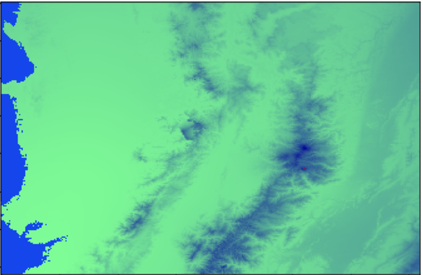
\includegraphics[scale=1]{tmax_picture_1}
	\caption{\label{tmax_picture} Mise sous forme graphique du tableau des température maximales pour le mois de janvier 2011 }
\end{figure}

\paragraph{Contexte climatique Colombien}La Colombie se trouvant à proximité de l'équateur, on y trouve que deux saisons: l'été ou saison sèche (de décembre à janvier et de juillet à août) puis l'hiver ou saison des pluies (d'avril à mai et de octobre à novembre). Le relief du pays ainsi que sa taille, font varier le climat de chaud et humide pour la partie amazonienne et la région des caraïbes, désertique pour la région de Guajira tout au nord et glacial pour les zones en haute altitude à plus de 3000 mètres. Le département de Risaralda se trouve dans le centre de la Colombie dans la région de l'Axe du café et jouit de conditions climatiques, géographiques et géologiques idéales pour la culture du café. Les températures oscillent entre 8 et 24 degrés mais un phénomène appelé \textit{El Niño} perturbe régulièrement le climat à l'échelle du continent. 

% http://www.actulatino.com/2016/01/14/colombie-el-nino-provoque-chaleur-et-secheresse-juan-manuel-santos-appelle-a-la-vigilance/

% https://public.wmo.int/fr/medias/communiqu%C3%A9s-de-presse/d%E2%80%99une-intensit%C3%A9-exceptionnelle-l%E2%80%99%C3%A9pisode-el-ni%C3%B1o-amorc%C3%A9-son-d%C3%A9clin-mais


\paragraph{El Niño}El Niño désigne un phénomène climatique qui se caractérise par une augmentation des températures de l'eau dans l'est du Pacifique sud due à une perturbation dans la circulation atmosphérique entre les pôles et l'équateur. Ces perturbations déplacent les zones de précipitations, modifient les routes des cyclones ou typhons provoquent à certains endroits de fortes précipitations et à d'autres de longues périodes de sécheresse. Même dans les zones tempérées, les périodes El Niño changent les habitudes climatiques. Durant l'été austral 2015-2016 s'est produit un des épisodes El Niño le plus fort jamais enregistré\cite{OMM}. Si une grande partie de l'Amérique du Sud a été victime de fortes précipitations, la Colombie, elle, a subit une longue période de sécheresse et l'Europe a connu des records de chaleur. Sur la figure \ref{Nino} on peut observer les différents pics correspondants à l'intensité du phénomène ainsi que pour son opposé, La Niña. 

\begin{figure}[H]
	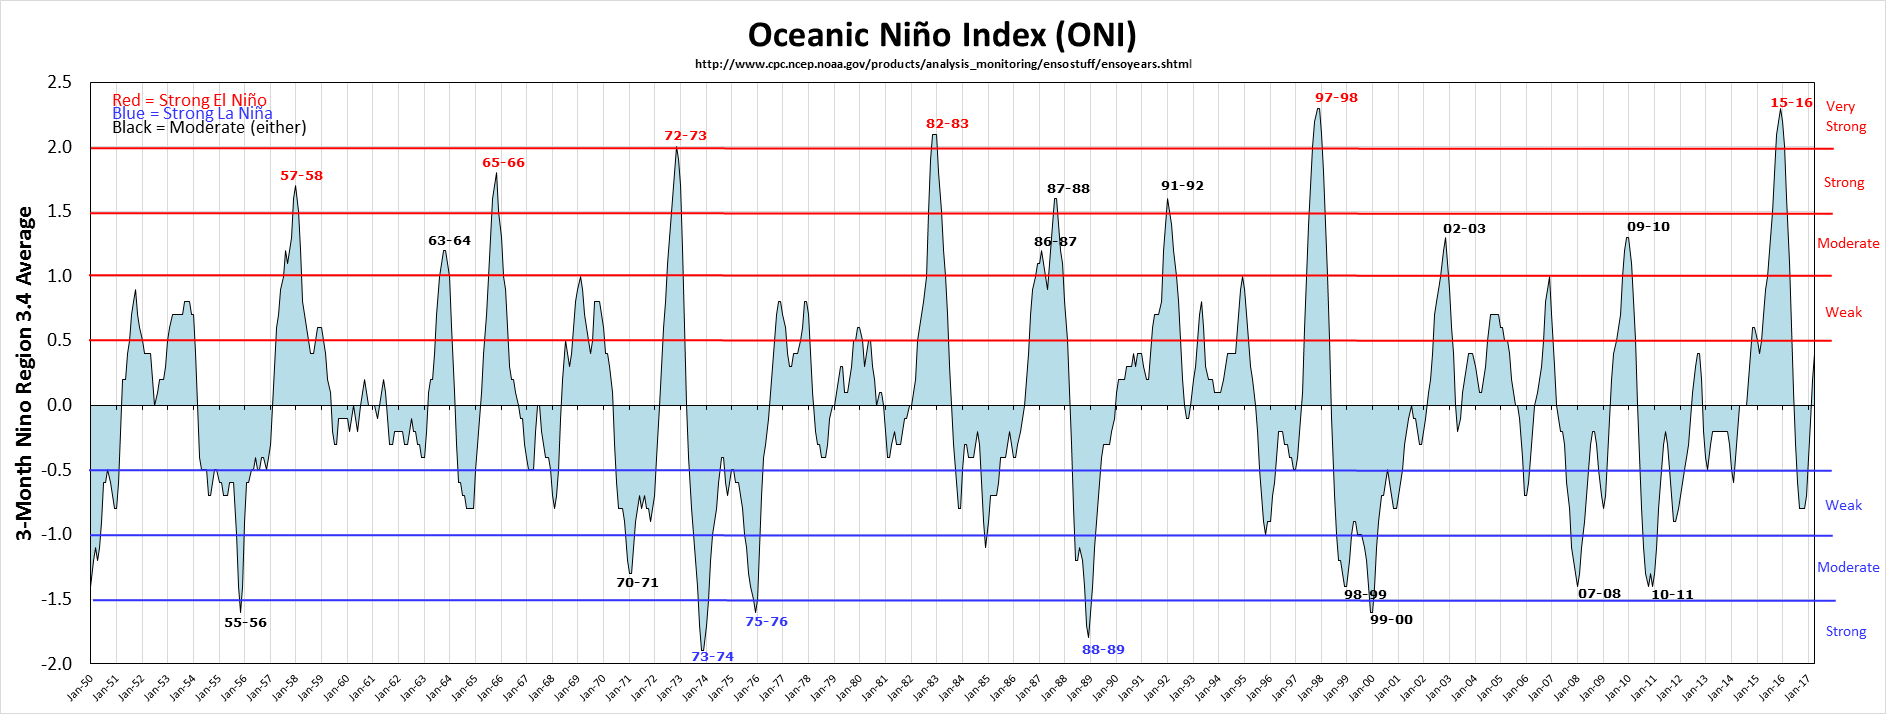
\includegraphics[scale=0.25]{VariationElNino}
	\caption{\label{Nino} Intensité du phénomène El Niño au cours des ans\newline Source: \textit{http://ggweather.com/enso/oni.htm}}
\end{figure}

\paragraph{Impact du réchauffement climatique} Outre les phases d'El Niño, il est nécessaire de rappeler que le climat mondiale se réchauffe et que des conséquences se font ressentir. Le Centre du Commerce International \cite{CCI} nous donne un aperçu des conséquences que ce réchauffement pourrait avoir pour la Colombie. "Les coûts de production sont susceptibles d'augmenter en raison des nouvelles conditions climatiques favorisant la prolifération des insectes, invasions et microbes pathogènes, et perturbant à l'équilibre naturel entre certains parasites et leurs prédateurs naturels. Les maladies se développeront vers de nouvelles zones. Les besoins en eau peuvent augmenter en raison de températures plus élevées causant plus d'évaporation, forçant de nombreux agriculteurs à recourir à l'irrigation. Dans certaines régions, les agriculteurs voudront transférer leur production de café à de plus hautes altitudes afin de chercher d'un meilleur environnement."(Guide de l'Exportateur de Café, CCI, 2011 \cite{GuideCafe})


\subsection{Données de sols} 
Les données de qualité de sol sont subdivisées en profils. Chaque profil est séparé en une ou plusieurs couches d’une certaine profondeur dont sont renseignées les caractéristiques comme le pH, la texture ou encore le taux de matière organique. Les différentes textures sont présentées sur la figure \ref{TriangleTexture}. Afin d'avoir des données uniformes, les moyennes sur les 3 premières couches jusqu'à 1 mètre de profondeur ont été réalisées pour le pH et le niveau de matière organique alors que pour la texture, la somme des variable binaire a été effectuée. \\


\noindent Les données proviennent d'un GIS (Geographical Information System), d'où il a été possible de croiser les données point par point afin d'extraire le profil de sol correspondant à un set de coordonnées GPS. Malheureusement les profils ne contiennent que pH, matière organique et texture. Des données très hétérogènes contenaient d'autres informations sur la composition chimique du sol mais leur structure et leur répartition irrégulière dans la zone de travail ont forcé à abandonner leur utilisation par manque de temps et de ressources.

% triangulo-del-suelo
\begin{figure}[H]
	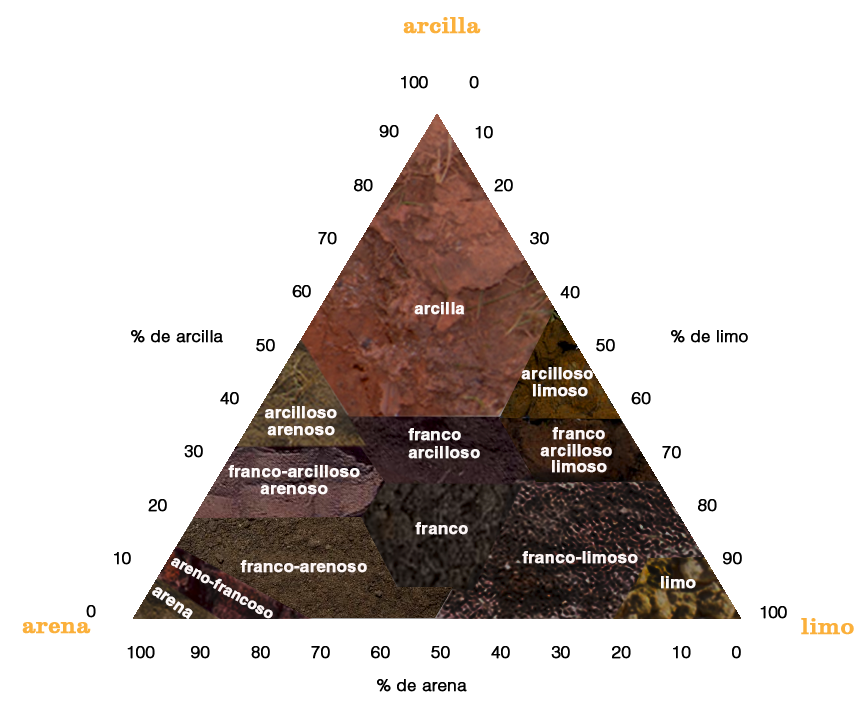
\includegraphics[scale=0.7]{triangulo-del-suelo}
	\caption{\label{TriangleTexture} Triangle représentant les différentes textures de sols\newline Source: \textit{http://www.construnatura.com/esp/articulo/agricultura-ecol-gica/el-suelo-como-fuente-de-vida--propiedades--ii-}}
\end{figure}






%################################################################################################################

\chapter{Méthodes de modélisation}
\section{Rappel des objectifs}\label{obj}
Ce projet a deux principaux objectifs. Le premier est de trouver s'il existe différents groupes de café ayant des relations entre les conditions de culture et les caractéristiques physiques ou sensorielles. On cherche donc dans cette première partie à caractériser les cafés. On peut ici parler de clustering.  Le second objectif serait de prédire les caractéristiques physiques ou sensorielles à partir des données sur les conditions de culture. Nous avons donc ici plusieurs possibilités de manières d'agir. Par exemple, si le clustering a réussi à diviser les cafés en différentes classes, on cherchera à prédire dans quelle classe se situe un nouveau café. Plus spécifiquement, on pourra se concentrer sur certains attributs du café, par exemple l'acidité, afin d'estimer quelle sera la note attribuée. 



\newpage

\section{Apprentissage supervisé}
% knn, réseaux de neurones etc
Le but de l'apprentissage supervisé est d'expliquer des sorties (outputs) à partir d'entrées (inputs). Des règles sont calculées à partir de données d'apprentissage selon différents modèles. Par la suite, le modèle est utilisé pour catégoriser des nouvelles données. On essayera ici d'expliquer les données gustatives du café ou ses défauts physiques à l'aide des données climatiques et de sols. 


\subsection{Random Forest}

La méthode Random Forest, ou \textit{forêts d'arbres décisionnels} en français, fait partie des méthodes ensemblistes\cite{EnsembleMethods}, qui utilisent la combinaison de plusieurs modèles de base, d'apprentissage automatique. Elle combine les concepts de sous-espaces aléatoires et de bagging.\\

\noindent Le bagging\label{bagging}, ou \textit{bootstrap agregation}, consiste à sous-échantillonner (ou ré-échantillonner au hasard avec doublons) le set d'entrainement et de faire générer à l’algorithme voulu un modèle pour chaque sous-échantillon. On utilise le bagging pour réduire la variance de la fonction de prédiction estimée. Le bagging semble bien fonctionner pour les procédures avec une grande variance et un petit biais, comme les arbres de décision. \cite{hastie_09_elements-of.statistical-learning}\\


\noindent Random Forest effectue donc un apprentissage sur de multiples arbres de décision entraînés sur des sous-ensembles de données légèrement différents \cite{Statistics01randomforests}.


\begin{figure}[H]
	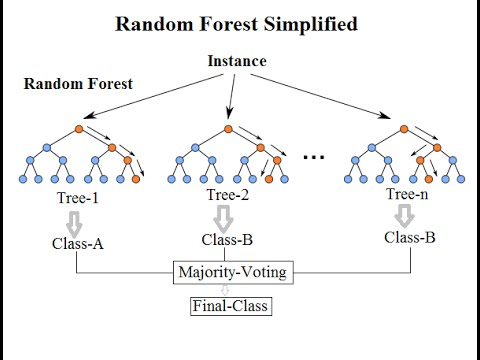
\includegraphics[scale=0.7]{RandomForestSimple}
	\caption{\label{RandomForestSchema} Schéma simple du fonctionnement de Random Forest. \newline Source: \textit{https://www.youtube.com/watch?v=ajTc5y3OqSQ}}
\end{figure}

\subsection{Partial Least Square (PLS)} 

% https://www.youtube.com/watch?v=WKEGhyFx0Dg 
% https://www.utdallas.edu/~herve/abdi-wireCS-PLS2010.pdf 

PLS, originalement pour \textit{Partial Least Squares regression} puis plus récemment pour \textit{Projection to Latent Structures} est une méthode qui combine des propriétés de la PCA ainsi que de multiples régressions linéaires. Au lieu de trouver un hyperplan de la variance maximale, entre les variables dépendantes et indépendantes, cette méthode va trouver un modèle de régression linéaire en projetant les variables indépendantes et dépendantes dans un nouvel espace. Ce sont les variables latentes. Cette méthode est particulièrement utile lorsqu'il est nécessaire de prédire un jeu de variables dépendantes à partir d'un très grand jeu de variables indépendantes.  

\begin{figure}[H] 
	\centering
	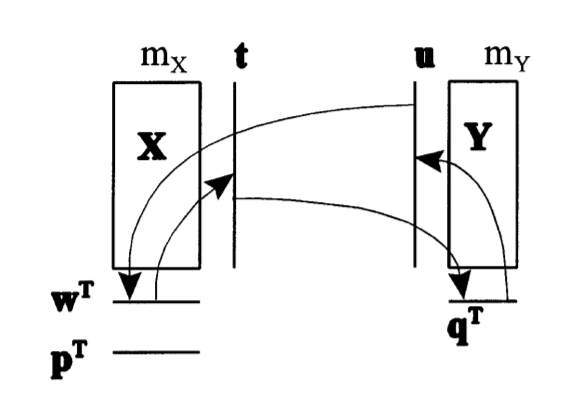
\includegraphics[scale=0.5]{PLS_1} 
	\caption{\label{PLSschema}Méthode PLS. X est représenté par son score t et Y par u. Une première estimation de U est multipliée à travers X pour obtenir une aproximation du poid $ \omega_t $. Le poid est normalisé pour être de longueur 1 et remultiplié à travers X pour produire t. A partir de t et de Y, le poid $ q^T $ est obtenu ce qui donne un nouveau vecteur u. Cette opération est répétée jusqu'à la convergence de t.\cite{CEM:CEM515}} 
	% http://www.umb.no/statisk/specmod/mbseminar/Westerhuis1998.pdf 
\end{figure} 

\subsection{Multi Block PLS} 
% http://www.models.life.ku.dk/~courses/MBtoolbox/pres_IntroMultiBlock.pdf 

% https://books.google.ch/books?id=PPUbvBUvmWoC 

% http://www.umb.no/statisk/specmod/mbseminar/Westerhuis1998.pdf 

La PLS multi block est une extension de la méthode PLS qui sépare les variables indépendantes en plusieurs blocks afin de leur donner une plus grande interpértabilité et plus d'informations sur la structure générale des données. Dans le cadre de ce projet, on peut imaginer séparer les données climatiques des données de sol par exemple.   
L'exécution est très similaire à la méthode PLS classique.  

\begin{figure}[H] 
	\centering
	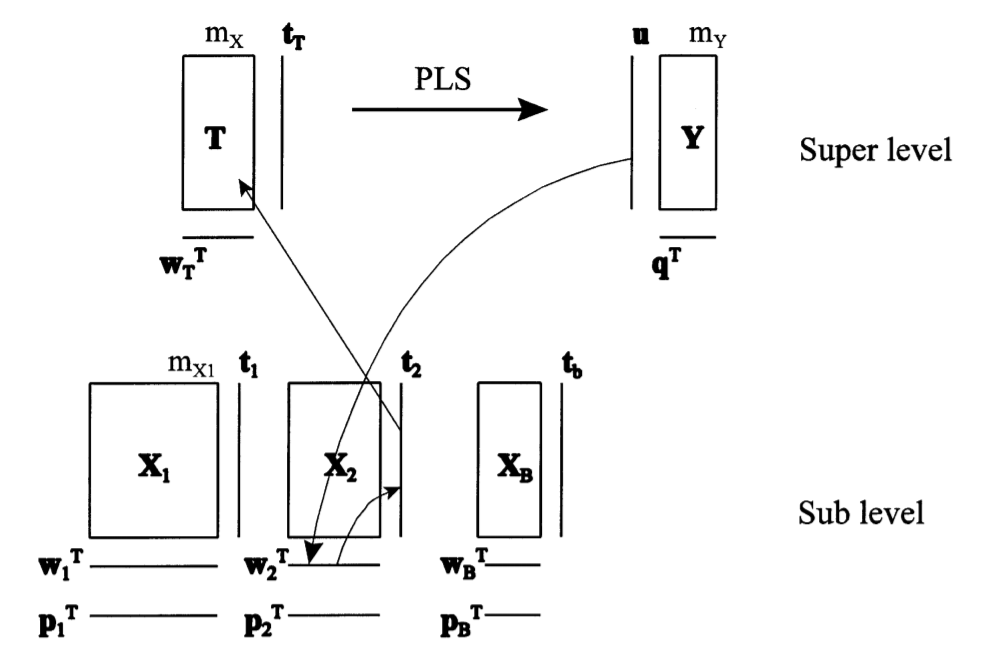
\includegraphics[scale=0.5]{MBPLS_1} 
	\caption{\label{MBPLSschema} Méthode MBPLS. Un score de départ u est régressé sur tous les blocs $ X_b $ pour donner les poids variables du bloc $ w^T_b $ Les poids des variables de blocs sont normalisés à la longueur un et multipliés par les blocs pour donner les scores de blocs $ t_b $.  Les scores de blocs sont combinés dans le super bloc T. Un cycle PLS entre T et Y est effectué pour donner le poids superieur $ W^T_T $, qui est également normalisé à la longueur un, et le super score $ t_T $. L'opération est répétée jusqu'à la convergence de $ t_T $. \cite{CEM:CEM515}} 
	% http://www.umb.no/statisk/specmod/mbseminar/Westerhuis1998.pdf 
\end{figure} 






\newpage

\section{Apprentissage non-supervisé}
Contrairement à l'apprentissage supervisé, l'apprentissage non-supervisé tente de trouver des groupes dans des données hétérogènes. Le but est d'extraire des connaissances à partir de ces données. Comme mentionné dans la partie \ref{obj}, notre but est de découvrir différents groupes de café identifiables. 


\subsection{SOM}

Les différentes classes gustatives d'un café peuvent être considérées comme des entrées afin vérifier s'il est possible de regrouper différents cafés qui se distingueraient. Afin de trouver les différentes catégories de café, nous testerons les capacités de l'algorithme SOM (pour Self Organizing Map ou Cartes Auto Adaptatives en français) qui utilise un réseau de neurones pour étudier la répartition des données dans un espace de grande dimension. 

\noindent Un bel exemple de SOM est celui de la carte de la pauvreté mondiale réalisé par le \textit{Department of Computer Science and Engineering} de l'université \textit{Helsinki University of Technology}. 

\begin{figure}[H]
	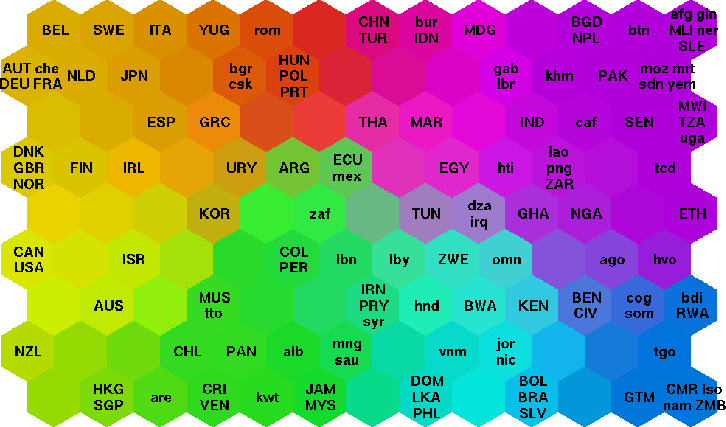
\includegraphics[scale=0.5]{SOMWordlPovertyMap}
	\caption{\label{SOMPovertyMap} Pays organisés en SOM d'après des indicateurs de pauvreté. \newline Source: \textit{http://www.cis.hut.fi/research/som-research/worldmap.html}}
\end{figure}

\begin{figure}[H]
	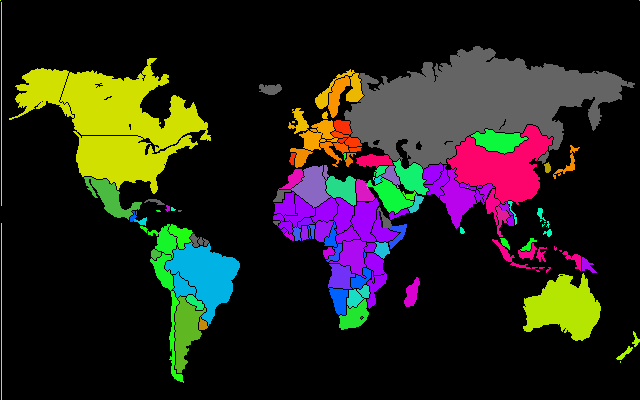
\includegraphics[scale=0.55]{worldmap}
	\caption{\label{WorldPovertyMap} Pays correspondants à la carte SOM de la figure \ref{SOMPovertyMap} \newline Source: \textit{http://www.cis.hut.fi/research/som-research/worldmap.html}}
\end{figure}




% TODO - supprimer ou pas ? c'est chiant la théorie on veut des résultats

\newpage
\section{Optimisation}

\subsection{Boosting}
Le principe du boosting est quelque peu différent du bagging (voir section \ref{bagging}). Les différents classifieurs sont pondérés de manière à ce qu’à chaque prédiction, les classificateurs ayant prédit correctement auront un poids plus fort que ceux dont la prédiction est incorrecte.\\


\noindent Adaboost est un algorithme de boosting qui s’appuie sur ce principe, avec un paramètre de mise à jour adaptatif permettant de donner plus d’importance aux valeurs difficiles à prédire, donc en boostant les classificateurs qui réussissent quand d’autres ont échoué. Des variantes permettent de l’étendre à la classification multiclasses. Adaboost s’appuie sur des classificateurs existants et cherche à leur affecter les bons poids vis à vis de leurs performances\cite{EnsembleMethods}.\\


\begin{figure}[H]
	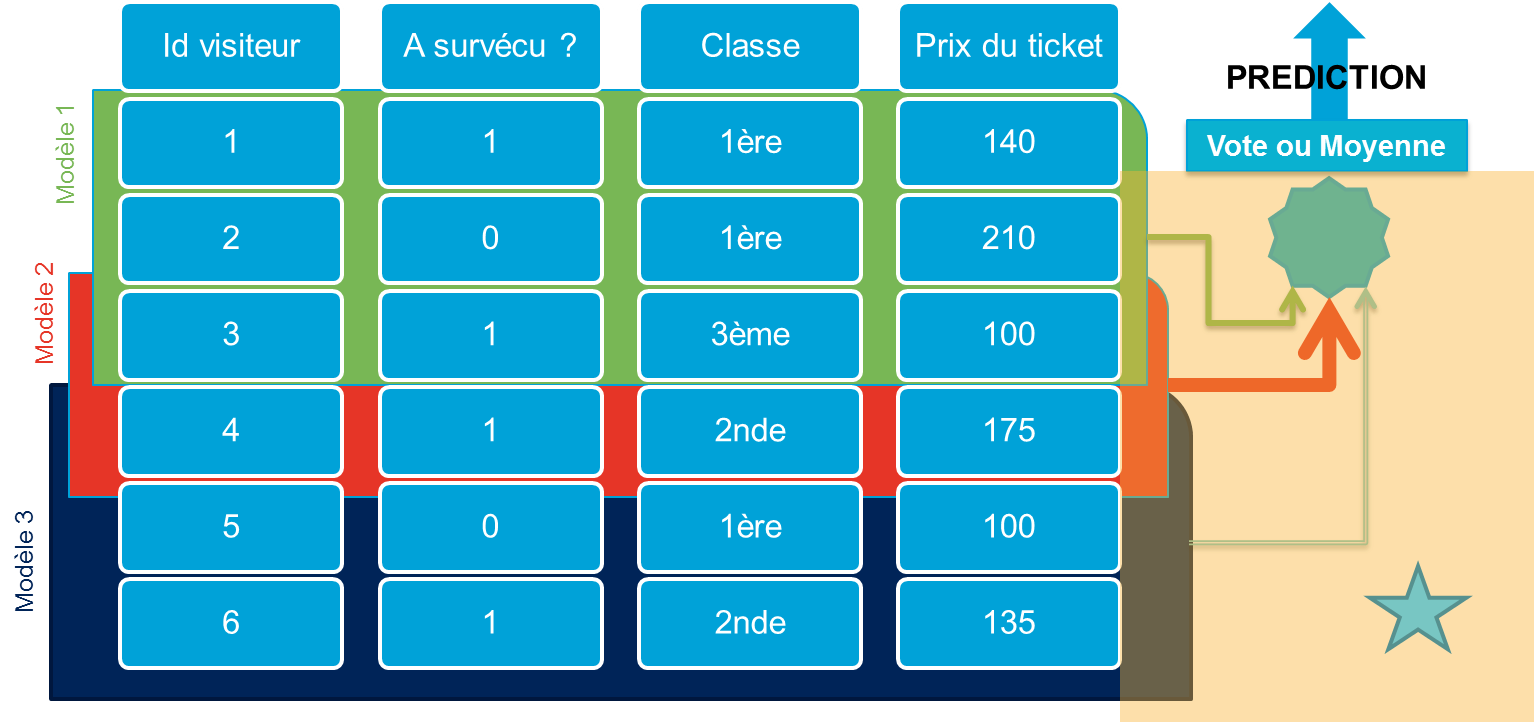
\includegraphics[scale=0.5]{boosting1}
	\caption{\label{BoostingSchema}Schéma du fonctionnement du Boosting \newline Source: \textit{http://www.cis.hut.fi/research/som-research/worldmap.html}}
\end{figure}

\noindent Gradient Boosting est une méthode de machine learning utilisée pour les problèmes de classification et de régression. Elle fait aussi partie des méthodes ensemblistes, et est utilisée majoritairement avec des arbres de décision. L'idées est encore d'agréger plusieurs classificateurs ensemble mais cette fois en les créant itérativement.\\


\noindent Le classifieur du gradient boosting est donc au final paramétré par les poids de pondération des différents mini-classifieurs, ainsi que par les paramètres des fonctions utilisées. Il s’agit donc d’explorer un espace de fonctions simples par une descente de gradient sur l’erreur\cite{EnsembleMethods}.

\subsection{Cross-Validation}

Contrairement au bagging qui est utilisé pour réduire l'overfitting en entrainant plusieurs modèles sur des données ré échantillonnées (avec répétition) puis en construisant un modèle sur la moyenne de ces modèles, la cross-validation est utilisée pour tester la fiabilité d'un modèle en se basant sur un échantillonnage des données d'entrainement et de test. Il existe plusieurs méthodes: « holdout method », « k-fold cross-validation » et « leave-one-out cross-validation ».\\

\noindent La première consiste à diviser le set de données en deux et en utilisant une partie pour entrainer le modèle puis une autre pour le tester. L'erreur est estimée en calculant un score de performance avec une méthode comme MSE (Erreur Quadratique Moyenne ou \textit{Mean Square Error}). \\

\noindent Étant donné que les données sont souvent trop peu nombreuses pour se permettre de laisser tomber dès le départ une partie des données, la k-fold cross-validation devient utile. On divise le set en k échantillons puis on en sélectionne un comme étant le set de test puis les k-1 autres comme étant le set d'entrainement. On répète l'opération en sélectionnant chaque fois un échantillon différent pour le test. Le score de performance est calculé en réalisant la moyenne des scores des k validations effectuées. La méthode « Leave-one out » utilise le même principe mais en ne laissant qu'une seule entrée en dehors du set d'entrainement à chaque tour\cite{hastie_09_elements-of.statistical-learning}. 



	
	
\end{document}